\chapter{Digital Image Formation}
\label{ch:dif}

\section{Optical Systems}
As was described in chapter \ref{ch:hvs}, digital cameras, to some extent, try to mimic the behaviour of the human eye. This is achieved by a combination of optical elements, such as lenses and prisms, mechanical elements such as the shutter and digital circuits such as the imaging sensor. 

Figure \ref{fig:optics} describes a basic ray diagram of image formation. An image of the object at distance $d_0$ is projected to the image plane at distance $d_i$, where the image recording material is placed. As the two rays coming from an object cross at the location of the image, the resulting image is said to be in focus. Shown in the figure are also the focal points $F$ and $F'$, which denote the location where parallel rays cross the optical axis. For an object at infinity, this is also where the object would appear in focus on the image plane.

In modern digital cameras, the ray diagram consists of a multitude of different lens elements of different shapes, which can be moved to focus at different distances. In addition, optical low-pass filters are also used to prevent aliasing at the image sensor.

\begin{figure}
\centering
\begin{tikzpicture}
    % Optical Axis
    \draw[->] (-4,0) -- (8,0) node[right] {Optical Axis};
    
    % Object
    \draw[thick] (-2,0) -- (-2,2) node[midway,left] {Object};
    
    % Lens
    \draw[thick] (0,-3) -- (0,3);
    \draw[->] (0,-3.2) -- (0,3.2) node[midway, xshift=0.5cm, yshift=0.5cm] {Lens};    
    % Focal Points
    \fill[red] (3,0) circle (2pt) node[below] {$F$};
    \fill[red] (-3,0) circle (2pt) node[below] {$F'$};
    
    % Image
    \draw[thick,blue] (4,0) -- (4,-1.5) node[midway,right] {Image};
    
    % Distance indicators
    \draw[<->, black] (-2, 2.5) -- (0, 2.5) node[midway, above] {$d_o$};
    \draw[<->, black] (0, 2.5  ) -- (4, 2.5) node[midway, above] {$d_i$};
    
    % Rays
    % Ray parallel to optical axis
    \draw[->,red] (-2,2) -- (0,2);
    \draw[->,red] (0,2) -- (3,0);
    \draw[->,red] (3,0) -- (4,-1.5);
    
    % Ray through F
    \draw[->,green] (-2,2) -- (0,0);
    \draw[->,green] (0,0) -- (4,-1.5);
    
\end{tikzpicture}

\caption{Basic image formation example}
\label{fig:optics}
\end{figure}

\section{Image sensors}

In the analogue era, photographic film was used to produce images, but it was slow due to the development process that had to be applied post-photography. Nowadays, the photosensitive material used is usually a digital sensor, which can convert incoming photons to electrons, resulting in an electric charge. This is done by densely placing photosensitive sensors, so-called pixels, in a grid-like manner inside the image sensor. 

The resulting electric charge from the photons can then be converted to a digital value with an analog-to-digital converter (ADC). Each photosensor then registers its digital value.


\subsection{Color Imaging}
\label{ss:color}

Image sensors themselves are not able to sense colour, as they only detect the intensity of the light incident on itself from the photon, but are unable to read the wavelength of the photon. Information is thus lost, and alternative solutions have to be invented.

The most common solution is to use an optical colour filter array (CFA), which forms a similar grid as the image sensor, but instead, filters light by its wavelength. Colour can then be detected by designing the filters so that they only allow light in the red, green or blue wavelength ranges. A common colour filter design is shown in figure \ref{fig:cfa}, where for each red and blue pixel there are two green pixels. This pattern is known as the Bayer filter after its inventor Bruce Bayer \cite{Bayer1976}.

The reason for using twice as many green pixels is because the human visual system is also more sensitive to the green wavelengths \cite[36]{Ramanath}. The spectral sensitivities of the Nikon D5100 digital single-lens reflex camera (DSLR), measured by \citeauthor{D5100NPL}, are shown in figure \ref{fig:d5100}. It is apparent, that since the green channel is relatively sensitive to all wavelengths, it would produce a higher response for an equal-energy illuminant than the other channels.

Similarly, as for the human visual system, the imaging sensor computes its response to the incoming light by integrating the product of the illuminant's power spectral distribution, spectral reflectance of the object and the spectral responsivity of the sensor for a given colour, over the wavelength range of interest.

\begin{align}
R = \int_{\lambda_{\text{min}}}^{\lambda_{\text{max}}} E(\lambda) R(\lambda) S_R(\lambda) \, d\lambda \\
G = \int_{\lambda_{\text{min}}}^{\lambda_{\text{max}}} E(\lambda) R(\lambda) S_G(\lambda) \, d\lambda \\
B = \int_{\lambda_{\text{min}}}^{\lambda_{\text{max}}} E(\lambda) R(\lambda) S_B(\lambda) \, d\lambda,
\end{align}

where $E(\lambda)$ is the spectral power distribution (SPD) of the illuminant, $R(\lambda)$ is the spectral reflectance of the imaged object and $S_T(\lambda)$ is the sensitivity of the sensor for tristimulus value $T$ (either $R$, $G$ or $B$). $\lambda_{\text{min}}$ and $\lambda_{\text{maxja }}$ are defined by the optical system, typically restricted to the visible range $\lambda_{\text{min}}=380$ nm and $\lambda_{\text{max}} = 780$ nm.




\begin{figure}
\centering

\begin{tikzpicture}

% Loop to draw the squares
\foreach \i in {0,1,2,3} {
    \foreach \j in {0,1,2,3} {
        \pgfmathtruncatemacro{\row}{mod(\i, 2)}
        \pgfmathtruncatemacro{\col}{mod(\j, 2)}
        
        % Choose color based on position
        \ifnum \row=0
            \ifnum \col=0
                \def\fillcolor{blue}
            \else
                \def\fillcolor{green}
            \fi
        \else
            \ifnum \col=0
                \def\fillcolor{green}
            \else
                \def\fillcolor{red}
            \fi
        \fi

        % Draw the square
        \fill[\fillcolor] (\i,\j) rectangle ++(1,1);
    }
}

\end{tikzpicture}
\caption{Color Filter Array}
\label{fig:cfa}
\end{figure}

\begin{figure}
    \centering
    \pdftooltip{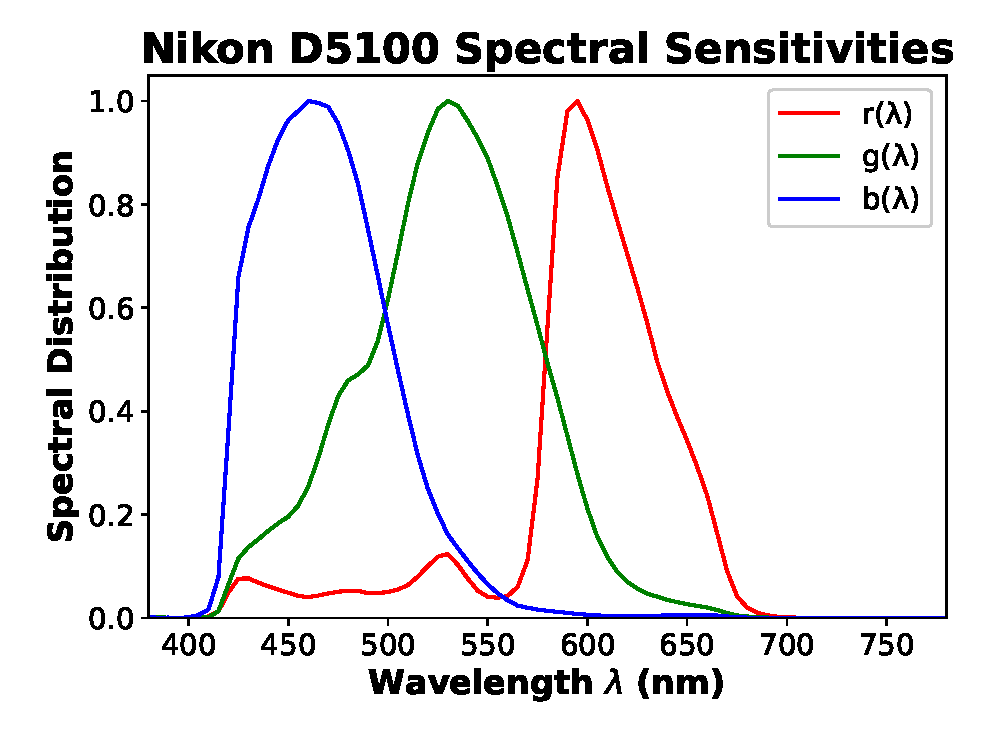
\includegraphics[width=\textwidth]{figures/d5100_rgb.eps}}{nikon}
    \caption{Nikon D5100 Spectral Sensitivities  \cite{D5100NPL}}
    \label{fig:d5100}
\end{figure}






\section{Color Image Processing Pipeline}

Producing a perceptually pleasing image involves several processing steps that are typically executed within the camera itself. These steps are orchestrated by a computing unit known as the Image Signal Processor (ISP). The tasks within the ISP are divided into distinct blocks, which can operate either in parallel or in series, depending on the specific processing requirements. Figure \ref{fig: dip} illustrates a typical colour image processing pipeline.

Each block in the pipeline has adjustable parameters that can be fine-tuned to meet specific preferences or requirements. Image quality experts are often utilized in the industry to optimize these parameters. 

\begin{figure}
\centering
\usetikzlibrary{shapes.geometric, arrows}

\tikzstyle{startstop} = [rectangle,
minimum width=3cm, 
minimum height=1cm,
text centered, 
draw=black, 
fill=red!30]

\tikzstyle{io} = [trapezium, 
trapezium stretches=true, % A later addition
trapezium left angle=70, 
trapezium right angle=110, 
minimum width=3cm, 
minimum height=1cm, text centered, 
draw=black, fill=blue!30]

\tikzstyle{process} = [rectangle, 
minimum width=3cm, 
minimum height=1cm, 
text centered, 
text width=3cm, 
draw=black, 
fill=orange!30]

\tikzstyle{decision} = [diamond, 
minimum width=3cm, 
minimum height=1cm, 
text centered, 
draw=black, 
fill=green!30]
\tikzstyle{arrow} = [thick,->,>=stealth]

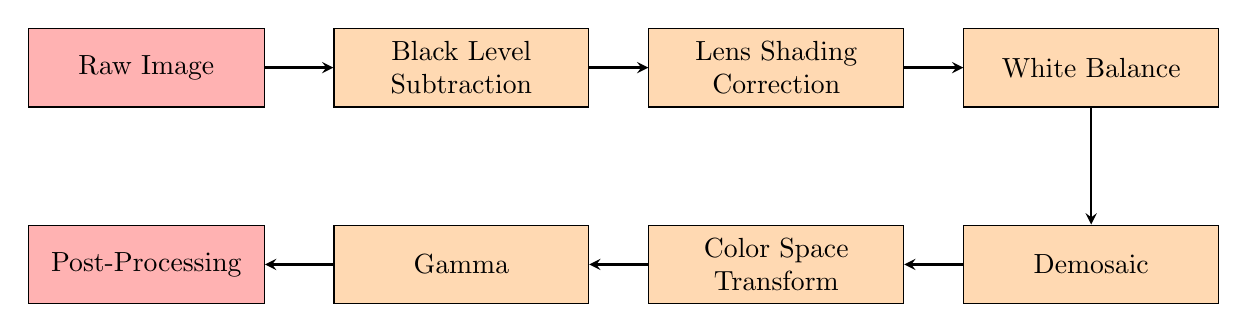
\begin{tikzpicture}[node distance=2cm]

\node (start) [startstop] {Raw Image};
\node (in1) [process, right of=start, xshift=2cm] {Black Level Subtraction};

\node (pro1) [process, right of=in1, xshift=2cm] {Lens Shading Correction};
\node (dec1) [process, right of=pro1, xshift=2cm] {White Balance};

\node (pro2a) [process, below of=dec1, yshift=-0.5cm] {Demosaic};

\node (pro2b) [process, left of=pro2a, xshift=-2cm] {Color Space Transform};
\node (pro2c) [process, left of=pro2b, xshift=-2cm] {Gamma};
\node (pro2d) [startstop, left of=pro2c, xshift=-2cm] {Post-Processing};



\draw [arrow] (start) -- (in1);
\draw [arrow] (in1) -- (pro1);
\draw [arrow] (pro1) -- (dec1);
\draw [arrow] (dec1) -- (pro2a);
\draw [arrow] (pro2a) -- (pro2b);
\draw [arrow] (pro2b) -- (pro2c);
\draw [arrow] (pro2c) -- (pro2d);

\end{tikzpicture}

\caption{Color Image Processing Pipeline. Adapted from \cite{Ramanath}, \cite{JianpingZhou2007IPTf}}
\label{fig:dip}
\end{figure}


\subsection{Pre-processing}

Pre-processing is a step that is different for each manufacturer, and is performed on a Bayer-format image, often called the raw image. Typically at least black level correction is performed at this stage, which attempts to remove dark noise from the image, which is caused by the conversion of thermal heat into electrons at the sensor. This type of noise can be characterized by taking images while the shutter is closed or by placing a lens cap in front of the camera so that no light enters inside and thus the noise source can be isolated \cite{Ramanath}.

\subsection{White Balance}

White balancing is a process employed in cameras to mimic the phenomena discussed in \ref{sec:chromaticadaptation}. This can be achieved by estimating the illuminant present in the scene and employing pre-defined multipliers to the pixel values that would make the red, green and blue responses equal for an object that appears white to a human. As each illuminant might result in different proportions of red, green and blue responses for an object that appears white to a human, these multipliers are often computed for a set of distinct illuminant types and interpolated accordingly to account for scenes with mixed illuminants. This process, combined with colour correction, cancels the effect of the illuminant and thus simulates the chromatic adaptation behaviour. \cite[ch.~4.6]{rowlands2020physics}

The accuracy of white balance algorithms is primarily determined by the illuminant estimation algorithm. A wrong estimation results in an improper choice of multipliers for both colour correction and white balance and results in a distinct tint in the output image. Thus the illuminant estimation process is perhaps the most important one in the colour processing pipeline. For a review on illuminant estimation algorithms, we refer the reader to \cite{colourconstancy}.

\subsection{Demosaic}

As discussed in Section \ref{ss:color}, producing color images begins with the image sensor being overlaid with a color filter array. This array allows only light of specific wavelengths to pass through, a concept illustrated in \ref{fig:cfa}. The next step in creating a full-colour image involves a crucial process known as demosaicing.

Demosaicing employs various interpolation techniques to achieve colour accuracy. Among the simplest is bilinear interpolation, which is based on direct interpolation methods. However, as documented in practical applications, these simple algorithms can sometimes fail, particularly at image edges \cite[46]{Ramanath}.

Acknowledging these limitations, researchers have developed more sophisticated algorithms. These advanced methods leverage cross-correlations between channels, adaptive filters, and frequency information. Such enhancements significantly improve the performance of demosaicing algorithms. For a more detailed discussion on this topic, interested readers may refer to \cite{gunturk2005demosaicking}.

\subsection{Colour Correction}

Figures \ref{fig:xyz} and \ref{fig:d5100} demonstrate the significant differences in spectral responsivities between the human eye and digital cameras, resulting in varying colour responses. Furthermore, the responsivities can vary across different units of the same camera module \cite{walowit2019best}. In addition to colour inaccuracy, it also results in observer metamerism, where two objects that appear the same colour to the human eye are captured differently by the camera.

To account for the differences, a colour correction matrix is typically applied to the input image. Often a 3x3 matrix is derived by regression from camera responses to known XYZ responses for a standard observer. \cite{rowlands2020color} Like white balancing, this matrix is unique to each illuminant as white balancing only guarantees that neutral colours are mapped correctly \cite{cheng2015beyond}. Furthermore, with colour correction matrices we can directly transform the input values to the desired output space, such as sRGB.

\subsection{Post-Processing}

Typically in subsequent steps, the goal is to make the image more pleasing to the viewer and comply with the desired output format.

